% path to figures directory
\graphicspath{{img/chapter_1/}}

\chapter{Introduction}
\label{chapter:introduction}

\begin{flushleft}
  \textit{\lipsum[1]}
\end{flushleft}

\section{The Standard Model and neutrinos}

Laboratory experiments to date have firmly established the predictive power of
the Standard Model (SM) of particle physics, a combined theory of the
electroweak and strong interactions described by the gauge group
$G_{\text{SM}} = \mathrm{SU}(3)_{c} \otimes \mathrm{SU}(2)_{L} \otimes \mathrm{U}(1)_{Y}$.
It is a model whose probes and predictions span at least 33 orders of
magnitude\footnote{The interval given is from the distance scales probed at the
  LHC (roughly $\SI{e-17}{\cm}$) to the size of the solar system (roughly
  \SI{e16}{\cm}).} with varying degrees of precision, and these are consistent
with almost all known experiments. Although it displays a number of arbitrary
features, the dynamics of the theory are mostly fixed by the fundamental
principles of gauge theory and Lorentz invariance. Most of this arbitrariness
resides in the matter sector of the theory, whose properties (masses, coupling
constants, quantum numbers, \textit{etc.}) are not predicted, but are instead
motivated on phenomenological grounds. We show the fields of the SM and their
defining properties in Table~\ref{tab:sm-fields}, according to the mathematical
conventions of Appendix~\ref{chapter:notation}.
\begin{table}[t]
  \centering
  \bgroup
  \def\arraystretch{1.3}% 1 is the default
  \begin{tabular}{ccc}
    \toprule
    Field                        & $\mathrm{SU}(3)_{c} \otimes \mathrm{SU}(2)_{L} \otimes \mathrm{U}(1)_{Y}$ & $\mathrm{SU}(2)_{+} \otimes \mathrm{SU}(2)_{-}$ \\
    \midrule
    $Q^{\alpha a i}$             & $(\mathbf{3}, \mathbf{2}, \tfrac{1}{6})$                                  & $(\mathbf{2}, \mathbf{1})$                      \\
    $L^{\alpha i}$               & $(\mathbf{1}, \mathbf{2}, -\tfrac{1}{2})$                                 & $(\mathbf{2}, \mathbf{1})$                      \\
    $\bar{u}^{\alpha}_a$                  & $(\bar{\mathbf{3}}, \mathbf{1}, -\tfrac{2}{3})$                           & $(\mathbf{2}, \mathbf{1})$                      \\
    $\bar{d}^{\alpha}_a$                  & $(\bar{\mathbf{3}}, \mathbf{1}, \tfrac{1}{3})$                            & $(\mathbf{2}, \mathbf{1})$                      \\
    $\bar{e}^{\alpha}$                    & $(\mathbf{1}, \mathbf{1}, 1)$                                             & $(\mathbf{2}, \mathbf{1})$                      \\
    $(G_{\alpha \beta})^a_{\ b}$ & $(\mathbf{8}, \mathbf{1}, 0)$                                             & $(\mathbf{3}, \mathbf{1})$                      \\
    $(W_{\alpha \beta})^i_{\ j}$ & $(\mathbf{1}, \mathbf{3}, 0)$                                             & $(\mathbf{3}, \mathbf{1})$                      \\
    $B_{\alpha \beta}$           & $(\mathbf{1}, \mathbf{1}, 0)$                                             & $(\mathbf{3}, \mathbf{1})$                      \\
    $H^{i}$                      & $(\mathbf{1}, \mathbf{2}, \tfrac{1}{2})$                                  & $(\mathbf{1}, \mathbf{1})$                      \\
    \bottomrule
  \end{tabular}
  \egroup
  \caption{The SM fields and their transformation properties under the SM gauge
    group $G_{\text{SM}}$ and the Lorentz group written as
    $\mathrm{SU}(2)_{+} \otimes \mathrm{SU}(2)_{-}$. The final unbolded number
    in the 3-tuples of the $G_{\text{SM}}$ column represents the
    $\mathrm{U}(1)_Y$ charge of the field, normalised such that $Q = I_{3} + Y$.
    For the fermions a generational index has been suppressed. See
    Appendix~\ref{chapter:notation} for details about the mathematical notation
    used here and throughout this work.}
  \label{tab:sm-fields}
\end{table}

The SM inherits the experimental success of the
$\mathrm{SU}(2) \otimes \mathrm{U}(1)$ theory of the weak interactions, first
proposed by Glashow~\cite{} in 1961 as a possible underlying structure for
Fermi's theory of beta decay. Before the end of the same decade,
Weinberg~\cite{} and Salam~\cite{} had constructed the modern theory of leptons
based on the spontaneous breaking of
$\mathrm{SU}(2)_{L} \otimes \mathrm{U}(1)_{Y}$ to the electromagnetic symmetry.
Interestingly, it seems that these seminal papers went mostly unnoticed (see
Fig.~\ref{fig:blah}) until the early 1970s, when 't~Hooft proved the
renormalisability of spontaneously broken gauge theories~\cite{} as a graduate
student working under the supervision of Veltman. By the mid 1970s the framework
had been extended to include the quarks~\cite{} and the unbroken chromodynamic
group, which was successfully shown to reproduce the Bjorken scaling seen in
deep-inelastic-scattering experiments through asymptotic freedom~\cite{}.
\begin{figure}[t]
  \centering
  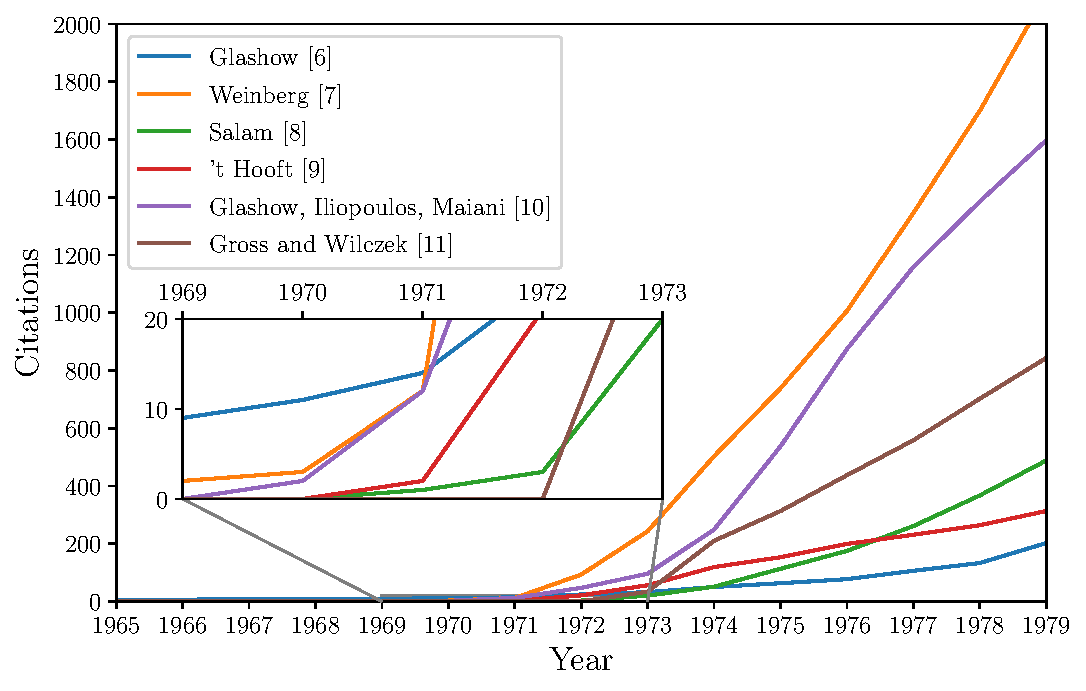
\includegraphics[width=\linewidth]{weinberg_citations}
  \caption{This is the caption}
  \label{fig:weinberg-citations}
\end{figure}

Despite its successes, the SM cannot be the complete theory of fundamental
particles and their interactions. It does not explain phenomena such as the
baryon asymmetry present in the Universe or its accelerating expansion.
Additionally, the particle spectrum contains no viable candidate for dark
matter, whose existence is strongly suggested by astrophysical and cosmological
data. The SM cannot explain why the electric dipole moment of the neutron is so
small, why there are three generations of matter or, notably in our case, the
origin of neutrino oscillations and their small but non-zero masses.

\section{Massive neutrinos in theory and experiment}

\lipsum[2]

\section{Effective field theories of the SM}

\lipsum[2]

\section{The flavour anomalies and their explanation}

\lipsum[2]

\myglossaryentry{lipsum}{lipsum}{Lorem Ipsum, a special type of fudge}{}
\myglossaryentry{dolor}{dolor}{No idea why}{parent={lipsum}}
\myglossaryentry{ibit}{ibit}{Sounds right, doesn't it?}{parent={lipsum}}
\myacronym{DFT}{density functional theory}
\myglossaryentry{$\pi$}{pi}{Greek letter pi, \ensuremath{\Pi} does this work?}{symbol={$\pi$}}
\myacronym{RDF}{radial distribution function}
\myglossaryentry{radial distribution function}{radialdistributionfunction}{}{symbol={$g(r)$}}
